\documentclass[11pt]{article}
\usepackage{amsmath, amssymb, amscd, amsthm, amsfonts}
\usepackage{graphicx}
\usepackage[hidelinks]{hyperref}

\oddsidemargin 0pt
\evensidemargin 0pt
\marginparwidth 40pt
\marginparsep 10pt
\topmargin -20pt
\headsep 10pt
\textheight 8.7in
\textwidth 6.65in
\linespread{1.2}

\title{\textbf{Time–Frequency and Statistical Analysis of GW150914 Using Open LIGO Data}}

\author{
	Sajjad Yami \thanks{All analysis code is publicly available at \url{https://github.com/cloner1998/gravitational-waves-LIGO}.}
	\\
	Course: Special Topics In Gravity \\
	Instructor: Dr. Bahram Mashhoon \\
	Institution: Sharif University of Technology \\
}

\date{\today}


\newtheorem{theorem}{Theorem}
\newtheorem{lemma}[theorem]{Lemma}
\newtheorem{conjecture}[theorem]{Conjecture}

\newcommand{\rr}{\mathbb{R}}

\newcommand{\al}{\alpha}
\DeclareMathOperator{\conv}{conv}
\DeclareMathOperator{\aff}{aff}

\begin{document}

\maketitle

\begin{abstract}
We present an independent analysis of GW150914 using publicly available LIGO strain data.
Through data conditioning, inter-detector cross-correlation, Q-transform time--frequency
analysis, and matched filtering against IMRPhenomD waveform templates, we reproduce the
key observational signatures of the first gravitational-wave detection. The measured
inter-detector time delay of $\Delta t \approx 7$\,ms, the characteristic chirp morphology
sweeping from $\sim$35\,Hz to $\sim$250\,Hz, and a reweighted signal-to-noise ratio of
$\hat{\rho} \approx 13.3$ with best-fit masses $m_1 = 35.5\,M_\odot$ and
$m_2 = 30.5\,M_\odot$ are all consistent with the published discovery results, confirming
the astrophysical origin of the signal.

\end{abstract}

\section{Introduction} \label{sec:1}

The detection of gravitational waves represents one of the most profound experimental achievements
in the history of physics. Predicted by Albert Einstein's general theory of relativity in 1916,
gravitational waves are ripples in the fabric of spacetime produced by the acceleration of massive
objects. For nearly a century, they remained beyond observational reach --- their amplitudes so
vanishingly small that detecting them demanded sensitivities previously thought impossible. That
barrier was broken on 14 September 2015, when the Laser Interferometer Gravitational-Wave
Observatory (LIGO) recorded GW150914, the first direct observation of a gravitational-wave signal,
originating from the inspiral and merger of two stellar-mass black holes approximately 1.3 billion
light-years away \cite{Abbott2016Discovery}. The event marked not merely a technological milestone but a
turning point in observational astronomy: it confirmed the existence of binary black hole systems,
validated general relativity in the strong-field dynamical regime, and opened an entirely new
observational window onto the universe, one inaccessible to electromagnetic astronomy.

\subsection*{Gravitational Waves from Linearized General Relativity}

Gravitational waves emerge naturally from Einstein's field equations when spacetime is treated as
a flat Minkowski background perturbed by a small metric deviation. Writing the full metric as
\begin{equation}
	g_{\mu\nu} = \eta_{\mu\nu} + h_{\mu\nu}, \qquad |h_{\mu\nu}| \ll 1,
\end{equation}
where $\eta_{\mu\nu} = \mathrm{diag}(-1,+1,+1,+1)$ is the flat Minkowski metric and $h_{\mu\nu}$
is the perturbation, and introducing the trace-reversed perturbation
\begin{equation}
	\bar{h}_{\mu\nu} = h_{\mu\nu} - \frac{1}{2}\,\eta_{\mu\nu}\, h, \qquad
	h \equiv \eta^{\mu\nu}h_{\mu\nu},
\end{equation}
the Lorenz gauge condition $\partial^{\mu}\bar{h}_{\mu\nu} = 0$ reduces the linearized Einstein
equations to the compact wave equation
\begin{equation}
	\Box\,\bar{h}_{\mu\nu} = -\frac{16\pi G}{c^{4}}\,T_{\mu\nu},
	\label{eq:wave}
\end{equation}
where $\Box = -c^{-2}\partial_t^2 + \nabla^2$ is the d'Alembertian operator and $T_{\mu\nu}$ is
the stress-energy tensor of the source. In vacuum ($T_{\mu\nu}=0$), Eq.~\eqref{eq:wave} becomes
the homogeneous wave equation, admitting plane-wave solutions propagating at the speed of light.
In the transverse-traceless (TT) gauge, only two independent polarization states survive --- the
\emph{plus} polarization $h_{+}$ and the \emph{cross} polarization $h_{\times}$ --- reflecting the
two physical degrees of freedom of a massless spin-2 field. A passing gravitational wave with
wavevector along the $z$-axis deforms a ring of test masses in the $xy$-plane as
\begin{equation}
	ds^2 = -c^2\,dt^2 + \bigl[1 + h_+(t)\bigr]\,dx^2
	+ \bigl[1 - h_+(t)\bigr]\,dy^2
	+ 2\,h_\times(t)\,dx\,dy + dz^2,
\end{equation}
making interferometric arm-length differences directly sensitive to the gravitational-wave strain
$h(t) = \Delta L(t)/L$.

\subsection*{The Quadrupole Formula and Binary Black Hole Systems}

Far from the source, the leading-order gravitational-wave emission is governed by the quadrupole
formula. The retarded solution to Eq.~\eqref{eq:wave} gives, in the TT gauge,
\begin{equation}
	h_{ij}^{\mathrm{TT}}(t,\mathbf{x}) =
	\frac{2G}{c^{4}\,r}\,\Lambda_{ij,kl}\,
	\ddot{Q}^{kl}\!\left(t_{\mathrm{ret}}\right), \qquad t_{\mathrm{ret}} = t - r/c,
	\label{eq:quad}
\end{equation}
where $r$ is the luminosity distance to the source, $\Lambda_{ij,kl}$ is the TT projection
operator, and $Q^{ij}$ is the traceless mass quadrupole moment\cite{Maggiore2007}
\begin{equation}
	Q^{ij} = \int_{\mathcal{V}} \rho\!\left(x^i x^j - \tfrac{1}{3}\,\delta^{ij} r^2\right)d^3x.
\end{equation}
Equation~\eqref{eq:quad} encodes a fundamental selection rule: gravitational-wave emission
requires a \emph{time-varying quadrupole moment}. Spherically symmetric collapse and uniformly
rotating rigid bodies produce no radiation; a binary system, by contrast, is an ideally
asymmetric and time-varying source.

For two point masses $m_1$ and $m_2$ in a circular Newtonian orbit of separation $d$ and
angular frequency $\Omega$, the total radiated power follows the Peters formula
\begin{equation}
	P = \frac{32}{5}\,\frac{G^4}{c^5}\,
	\frac{(m_1 m_2)^2(m_1+m_2)}{d^5}.
	\label{eq:peters}
\end{equation}
Energy loss through gravitational radiation causes the orbital separation to shrink and the
orbital frequency to increase. The merger timescale for a circular binary is
\begin{equation}
	\tau_{\mathrm{merge}} \approx
	\frac{12}{19}\,\frac{c^5\,d_0^4}{G^3\,m_1\,m_2\,(m_1+m_2)},
\end{equation}
where $d_0$ is the initial separation \cite{Maggiore2007}. For the GW150914 progenitor system this timescale was on
the order of the age of the universe, culminating in the observed merger event.

\subsection*{The Chirp Signal and the Chirp Mass}

The frequency evolution of the gravitational-wave signal during inspiral is governed by
\begin{equation}
	\dot{f}_{\mathrm{GW}} =
	\frac{96\pi^{8/3}}{5}\,
	\left(\frac{G\mathcal{M}}{c^3}\right)^{5/3}
	f_{\mathrm{GW}}^{\,11/3},
	\label{eq:fdot}
\end{equation}
where the \emph{chirp mass}
\begin{equation}
	\mathcal{M} = \frac{(m_1 m_2)^{3/5}}{(m_1+m_2)^{1/5}}
\end{equation}
is the single best-constrained quantity in a gravitational-wave observation.
Integrating Eq.~\eqref{eq:fdot} shows that $f_{\mathrm{GW}}$ increases monotonically with time,
and the waveform amplitude scales as $h \propto \mathcal{M}^{5/3} f_{\mathrm{GW}}^{2/3} / r$ \cite{Cutler_1994}.
The resulting signal --- a sinusoid with simultaneously increasing frequency and amplitude --- is
universally known as a \emph{chirp}. For GW150914, with $m_1 \approx 36\,M_\odot$ and
$m_2 \approx 29\,M_\odot$, the chirp mass is $\mathcal{M} \approx 28.3\,M_\odot$, and the
signal sweeps from $\sim 35$\,Hz to $\sim 250$\,Hz in roughly $0.2$ seconds \cite{Abbott2016Discovery}.

\subsection*{Three Phases of the Signal}

The complete gravitational-wave signal from a binary black hole coalescence divides into three
morphologically distinct phases:

\begin{enumerate}
	\item \textbf{Inspiral.} The early phase is well described by post-Newtonian (PN) perturbation
	theory, in which the binary slowly loses binding energy to gravitational radiation. The
	waveform is a chirp with monotonically increasing frequency and amplitude, whose phase
	evolution is captured order-by-order in the small parameter $v/c$. For GW150914, the
	inspiral sweeps through the LIGO band from $\sim 35$\,Hz to $\sim 150$\,Hz \cite{Cutler_1994, Maggiore2007}.
	
	\item \textbf{Merger.} As the separation approaches the light-ring radius, post-Newtonian
	expansions diverge and the system enters the fully nonlinear regime of general relativity.
	This phase, characterized by peak strain amplitude and highly asymmetric mass distribution,
	is accessible only through numerical relativity simulations, such as those underpinning the
	IMRPhenomD family of waveform models used in the present analysis\cite{Cutler_1994, Maggiore2007}.
	
	\item \textbf{Ringdown.} Following merger, the remnant Kerr black hole relaxes to stationarity
	by emitting gravitational radiation in the form of exponentially damped sinusoids known as
	quasi-normal modes (QNMs). The dominant QNM frequency and quality factor are determined
	entirely by the remnant mass $M_f$ and dimensionless spin $\chi_f$, providing a direct
	observational test of the Kerr no-hair theorem \cite{Cutler_1994, Maggiore2007}.
\end{enumerate}

\subsection*{Scope of This Work}

This paper presents an independent analysis of GW150914 using publicly available strain data from
the LIGO Open Science Center. The goal is to reproduce and interpret the key observational
signatures of the event through a sequence of complementary methods. We begin with data
acquisition and conditioning --- including power spectral density estimation, whitening, and
bandpass filtering --- to suppress instrumental noise and isolate the astrophysical signal
(Section~3). We then measure the inter-detector time delay between the Hanford (H1) and
Livingston (L1) observatories via cross-correlation, providing direct evidence of signal coherence
across the detector network (Section~4). A time--frequency analysis using the Q-transform is
employed to visualize the characteristic chirp morphology (Section~5). Finally, we apply matched
filtering with IMRPhenomD templates to quantify the signal-to-noise ratio, and perform a
$\chi^2$ signal consistency test to assess template match quality and suppress noise transients
(Section~6).

The combination of these analyses yields a reweighted SNR $\hat{\rho} \approx 13.3$, a reduced
$\chi^2_{\mathrm{red}} = 2.10$, and best-fit component masses of $35.5\,M_\odot$ and
$30.5\,M_\odot$, in close agreement with the published discovery paper \cite{Abbott2016Discovery}. Taken
together, they constitute a self-contained and reproducible confirmation of the first
gravitational-wave detection, and illustrate the power of open data in enabling independent
scientific verification.
\section{The LIGO Detectors and GW150914} \label{sec:2}
\subsection{Interferometric Detection of Gravitational Waves}

Gravitational waves are transverse perturbations of spacetime curvature that propagate at the speed of light. In the transverse–traceless (TT) gauge, a passing gravitational wave induces differential strain in orthogonal spatial directions. The observable quantity measured by ground-based detectors is the dimensionless strain
\begin{equation}
	h(t) = \frac{\Delta L(t)}{L},
\end{equation}
where $L$ is the interferometer arm length and $\Delta L(t)$ is the differential change in arm lengths induced by the gravitational wave\cite{Abbott2016Discovery}.

The Laser Interferometer Gravitational-Wave Observatory (LIGO) detectors are kilometer-scale Michelson interferometers with Fabry–Pérot arm cavities designed to measure strains on the order of $10^{-21}$. Each detector consists of two perpendicular 4 km arms. A passing gravitational wave stretches one arm while compressing the other, producing a measurable phase shift in the recombined laser light
\cite{Abbott2016Discovery}.

The strain sensitivity of LIGO is frequency-dependent and the most sensitive band is 100 to 300 Hz. At low frequencies, seismic noise dominates, while at high frequencies shot noise and quantum noise become significant. For binary black hole mergers such as GW150914, the majority of detectable signal power lies between approximately 30 Hz and 300 Hz, which motivates the frequency band used later in this analysis
\cite{Aasi2015AdvancedLIGO,Abbott2016Discovery}.
\subsection{The Hanford and Livingston Observatories}

LIGO operates two geographically separated detectors in the United States: the LIGO Hanford Observatory (H1) in Washington and the LIGO Livingston Observatory (L1) in Louisiana. The two observatories are separated by approximately 3000 km. This separation is essential for distinguishing true astrophysical signals from local instrumental or environmental disturbances \cite{Abbott2016Properties}.

A gravitational wave arriving from an astrophysical source will be observed in both detectors with a relative time delay determined by the source sky location, the orientation of each interferometer, and the propagation speed of gravitational waves (consistent with the speed of light)\cite{Abbott2016Properties}. Because the light travel time between the two sites is about 10 milliseconds, the maximum possible arrival time difference between H1 and L1 is approximately $\pm 10$ ms. Therefore, measuring an inter-detector delay within this range provides strong evidence for an astrophysical origin.

The detectors are not perfectly co-aligned; their antenna response patterns differ slightly due to their orientations. Consequently, the measured strain amplitudes in H1 and L1 are not identical, although the waveform morphology remains consistent\cite{Abbott2016Discovery}.

\begin{figure}[h]
	\centering
	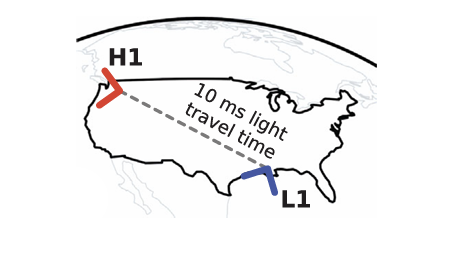
\includegraphics[width=0.4\textwidth]{figure/ligo_map}
	\caption{Geographic locations of the Hanford and Livingston observatories\cite{Abbott2016Discovery}.}
\end{figure}


\subsection{The Event GW150914}

The gravitational-wave event GW150914 was the first direct detection of gravitational waves, observed on 14 September 2015 at GPS time 1126259462.4. The signal originated from the merger of two stellar-mass black holes with component masses of approximately $36\,M_{\odot}$ and $29\,M_{\odot}$. The event marked the first direct observation of a binary black hole system and provided strong confirmation of general relativity in the strong-field regime\cite{Abbott2016Discovery, Abbott2016Properties}.

In the detector band, GW150914 appears as a short-duration chirp lasting roughly 0.2 seconds, with frequency sweeping from approximately 35 Hz to about 250 Hz. This characteristic frequency evolution makes the event well-suited for both time--frequency analysis and matched filtering techniques.

\subsection{Physical Expectations for the Present Analysis}

Before performing the data analysis, several physical expectations guide the interpretation:

\begin{enumerate}
	\item \textbf{Coincident detection:} The signal must appear in both H1 and L1.
	\item \textbf{Finite time delay:} The inter-detector delay should be less than 10 ms.
	\item \textbf{Chirp signature:} The signal should exhibit a monotonic increase in frequency over time.
	\item \textbf{Template consistency:} Matched filtering with a physically motivated waveform should yield a high signal-to-noise ratio (SNR).
	\item \textbf{Statistical consistency:} A chi-square test should indicate that the signal’s frequency content matches the theoretical template.
\end{enumerate}

The following sections evaluate these expectations using publicly available LIGO strain data.

\section{Data Acquisition and Conditioning} \label{sec:3}
\subsection{Open Data Retrieval}

The strain data used in this work were obtained from the LIGO Open Science Center (LOSC), which provides publicly available calibrated strain time series from the Advanced LIGO detectors. The data correspond to the event GW150914 at GPS time 1126259462.4.

For the primary analysis, a time window of $\pm 4$ seconds around the merger time was retrieved for both the Hanford (H1) and Livingston (L1) detectors. The strain time series is sampled at 4096 Hz in the public dataset, which is sufficient to resolve the frequency band of interest (30–300 Hz).

The strain $h(t)$ represents the dimensionless differential arm length variation,
\[
h(t) = \frac{\Delta L(t)}{L},
\]
where $L=4\,\mathrm{km}$ is the interferometer arm length.

The use of publicly released calibrated strain ensures reproducibility and consistency with the official analyses.

 
\begin{figure}[h]
	\centering
	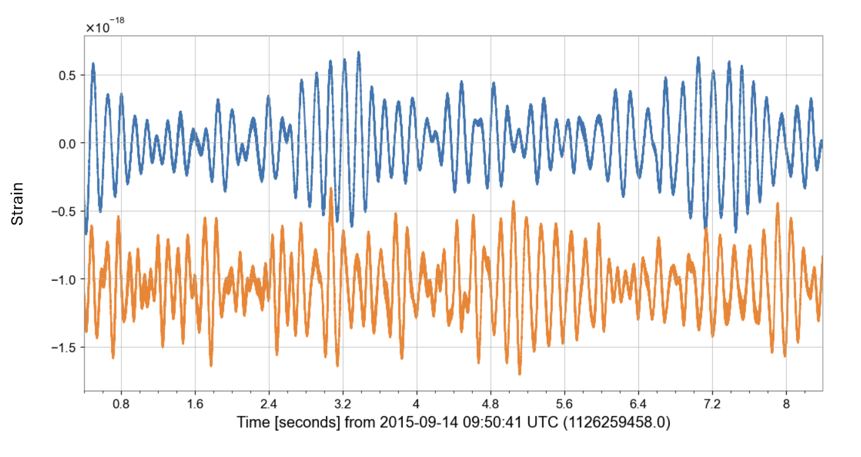
\includegraphics[width=0.85\textwidth]{figure/raw_strain.png}
	\caption{Raw strain data from H1 and L1 around GW150914 merger time (Blue: H1, Red: L1).}
\end{figure}


\subsection{Noise Characteristics and Power Spectral Density}

Gravitational-wave detectors operate in the presence of non-white, frequency-dependent noise. The statistical characterization of this noise is described by the one-sided power spectral density (PSD), $S_n(f)$, defined through
\[
\langle \tilde{n}(f)\tilde{n}^*(f') \rangle = \frac{1}{2} S_n(f)\delta(f-f'),
\]
where $\tilde{n}(f)$ is the Fourier transform of the detector noise.

The PSD is essential for optimal filtering because it quantifies the variance of noise as a function of frequency. In Advanced LIGO, the noise budget is dominated by seismic noise below $\sim 20$ Hz, thermal noise in the intermediate band, and quantum shot noise above several hundred Hz \cite{Aasi2015AdvancedLIGO}.

In this analysis, the PSD was estimated directly from the strain data  over a 8-second segment. The resulting PSD was interpolated to match the frequency resolution of the template waveforms and truncated at low frequencies to suppress spectral leakage. 

\begin{figure}[h]
	\centering
	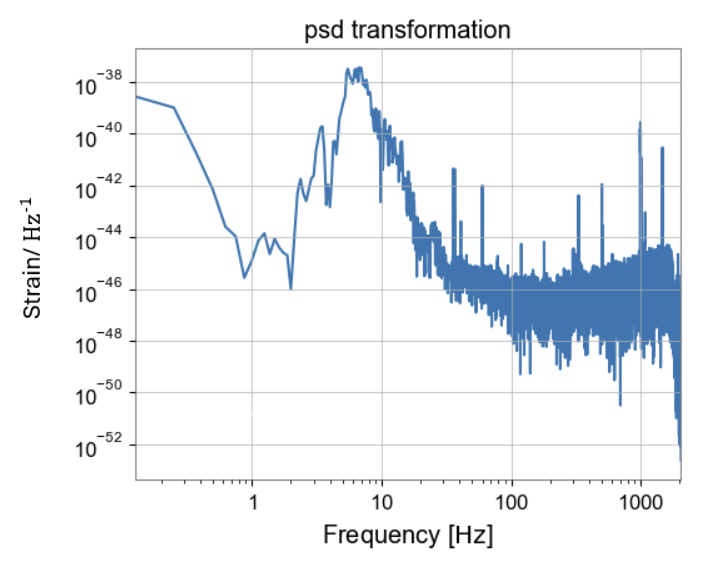
\includegraphics[width=0.8\textwidth]{figure/plot_psd.png}
	\caption{Estimated power spectral density of the H1 strain data.}
	\label{psd transformation}
\end{figure}


\subsection{Whitening Procedure}

Because detector noise is strongly frequency-dependent, direct time-domain analysis is essential. To equalize the noise variance across frequencies, the strain data were whitened by dividing the Fourier-domain data by the square root of the PSD:

\[
\tilde{h}_{\mathrm{white}}(f) = \frac{\tilde{h}(f)}{\sqrt{S_n(f)}}.
\]

This operation transforms colored noise into approximately unit-variance white noise. Whitening is essential for:

\begin{itemize}
	\item Visual identification of transient signals,
	\item Cross-correlation analysis between detectors,
	\item Time–frequency representations such as the Q-transform.
\end{itemize}

After whitening, the noise background becomes approximately stationary with uniform variance across frequencies.

\subsection{Bandpass and Notch Filtering}

Although whitening suppresses frequency-dependent noise, residual contributions outside the astrophysically relevant band remain. For binary black hole mergers similar to GW150914, most detectable signal power lies between approximately 30 Hz and 300 Hz. From fig \ref{psd transformation}, the best frequency window to study is something between 50 to 300 Hz\cite{Abbott2016Discovery,Abbott2016Properties}. 

Therefore, a bandpass filter between 50 Hz and 300 Hz was applied to the strain data. The lower cutoff reduces contamination from seismic and suspension noise, while the upper cutoff removes high-frequency shot noise.

In addition, a narrow notch filter at 60 Hz was applied to suppress contamination from power-line harmonics, which are a known environmental noise source in ground-based interferometers \cite{Aasi2015AdvancedLIGO}.

After bandpass and notch filtering, the waveform morphology of GW150914 becomes clearly visible in the time domain over a $\sim 2$ s interval surrounding the merger.


\begin{figure}[h]
	\centering
	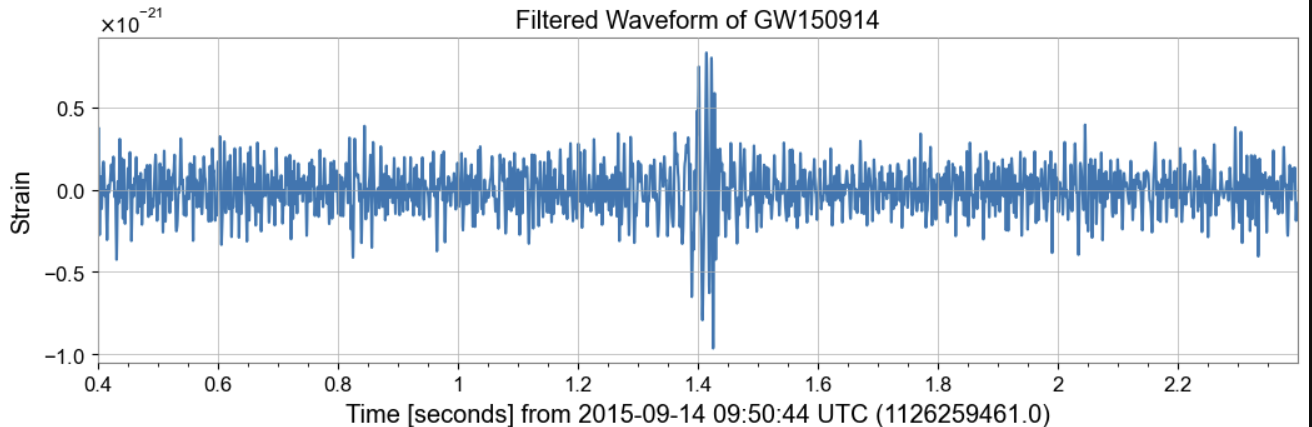
\includegraphics[width=0.85\textwidth]{figure/filtered_waveform}
	\caption{Bandpass and notch filtered strain signal near GW150914.}
	\label{filtered data}
\end{figure}


\subsection{Data Preparation for Subsequent Analysis}

Following conditioning, the strain data were cropped to shorter windows around the merger time for specific analyses:

\begin{itemize}
	\item $\pm 1$ ms window for cross-correlation time-delay measurement,
	\item $\pm 1$ s window for Q-transform analysis,
	\item $\pm 32$ s window for matched filtering and chi-square estimation.
\end{itemize}

Each time window was selected based on the statistical requirements of the corresponding method. Short windows minimize contamination from unrelated noise transients, while longer segments are necessary for stable PSD estimation and matched filtering.

This conditioned dataset forms the basis for the time-delay analysis presented in the next section.

\section{Time Delay Measurement Between H1 and L1 Detectors} \label{sec:4} 
\subsection{Method: Cross-Correlation}

A genuine astrophysical gravitational-wave signal must appear in both detectors with a time delay consistent with the light travel time between Hanford and Livingston (approximately $\pm 10$ ms). To measure this delay, the whitened and bandpass-filtered strain data from H1 and L1 were cross-correlated.

Given two discrete time series $h_H(t)$ and $h_L(t)$, the cross-correlation is defined as

\[
C(\tau) = \sum_{t} h_H(t) \, h_L(t+\tau),
\]

where $\tau$ is the time lag. The lag that maximizes $C(\tau)$ provides an estimate of the relative arrival time between the two detectors.

Prior to correlation, the Livingston data were multiplied by $-1$ to account for the relative detector orientation, which can invert the signal phase for certain sky locations.

The analysis was performed on a $\pm 1$ ms window around the merger time.


\begin{figure}[h]
	\centering
	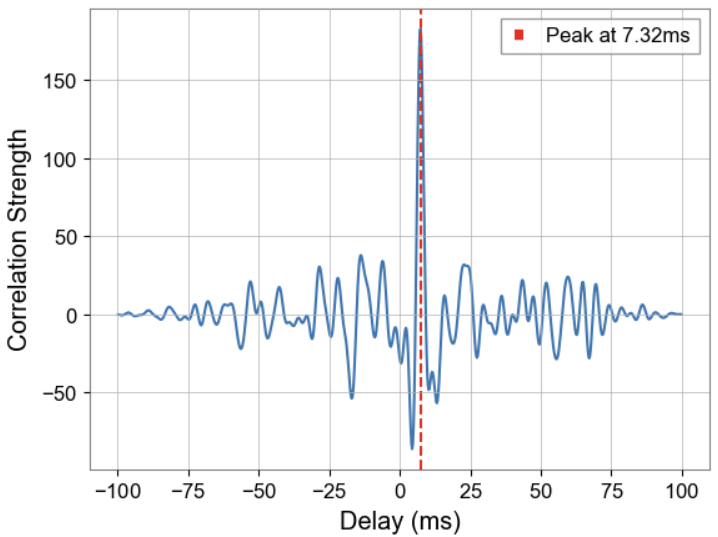
\includegraphics[width=0.6\textwidth]{figure/cross_correlation_peak}
	\caption{Cross-correlation between H1 and L1 showing a clear peak at the measured time delay.}
	\label{cross correlation}
\end{figure}

The cross-correlation exhibits a clear and statistically significant peak corresponding to a relative delay of

\[
\Delta t \approx \textbf{7} \ \text{ms}.
\]

This delay is well within the physically allowed range set by the 3000 km separation of the detectors. The sign of the delay indicates the direction of propagation across the detector network.

The presence of a sharp correlation peak strongly supports the interpretation of a coherent astrophysical signal observed by both interferometers.


\subsection{Off-Source Validation}

To assess the significance of the measured delay, the same procedure was applied to an off-source segment located 200 seconds away from the merger time. In this case, no dominant correlation peak was observed, and the inferred delay was consistent with random noise fluctuations.

\begin{figure}[h]
	\centering
	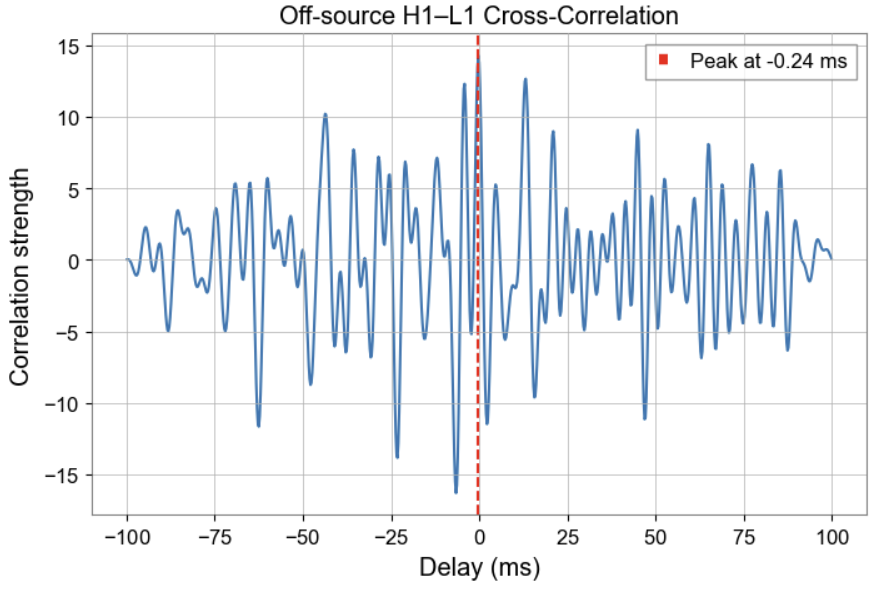
\includegraphics[width=0.6\textwidth]{figure/offsource_correlation}
	\caption{Cross-correlation in an off-source window showing no significant peak.}
	\label{off sourc cross correlation}
\end{figure}

The contrast between the on-source figure \ref{cross correlation} and off-source \ref{off sourc cross correlation} results demonstrates that the measured inter-detector delay at the merger time is not a generic feature of the noise but is associated with a transient coherent signal.

\subsection{Key Result}

The coincident detection of a transient signal in both detectors with a physically consistent time delay constitutes the first independent confirmation, within this analysis, that GW150914 is not a local instrumental artifact but a genuine gravitational-wave event.

\section{Time–Frequency Analysis (Q-Transform)} \label{sec:5}

\subsection{Q-Transform}
Time–frequency representation is useful
for visualizing transient gravitational-wave signals. For this purpose,
we use the Q-transform \cite{Chatterji2004,Chatterji2005}.

The Q-transformation is a windowed Fourier transform constructed using
Gaussian-windowed complex sinusoids with constant quality factor \( Q \).
For a strain time series \( h(t) \), it is defined as

\begin{equation}
	X(t_0, f_0) =
	\int_{-\infty}^{\infty}
	h(t)\,
	w_{t_0,f_0,Q}(t)\,
	e^{-2\pi i f_0 t}\, dt ,
\end{equation}

where \( w_{t_0,f_0,Q}(t) \) is a Gaussian window centered at time
\( t_0 \) and frequency \( f_0 \).

The quality factor is given by

\begin{equation}
	Q = \frac{f_0}{\Delta f},
\end{equation}

where \( \Delta f \) is the effective bandwidth. A larger \( Q \)
provides better frequency resolution but poorer time resolution,
while a smaller \( Q \) improves time localization at the expense
of frequency precision.

In gravitational-wave analysis, the Q-transform is commonly applied
to whitened strain data. For compact binary coalescences such as
GW150914, it reveals a characteristic chirp pattern: a signal
that increases in frequency and amplitude with time.

\subsection{Q-Transform Spectrogram}
To visualize the evolution of signal frequency with time, a time--frequency analysis was performed using a Q-transform spectrogram. 

The whitened and bandpass-filtered data in the range 30--300 Hz were used. The analysis window was centered on the merger time and extended $\pm 1$ s.


\begin{figure}[h]
	\centering
	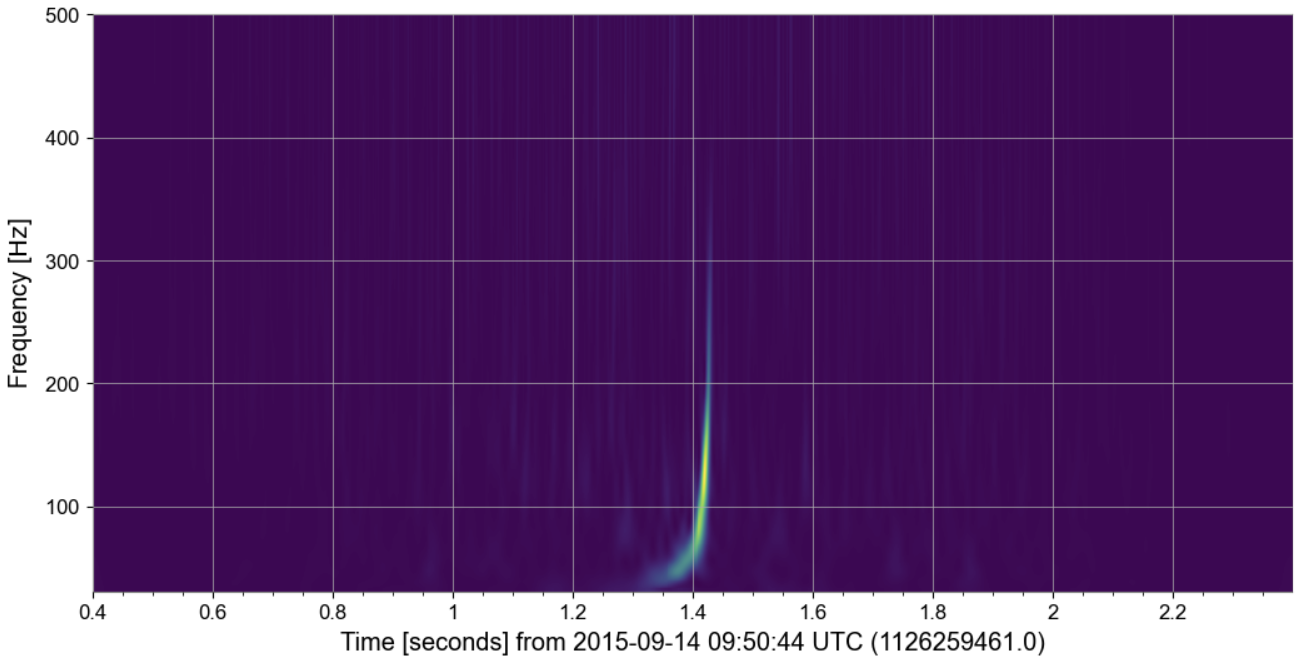
\includegraphics[width=0.9\textwidth]{figure/Qspectrogram}
	\caption{Time--frequency spectrogram of GW150914 showing the characteristic chirp structure.}
	\label{Qtransformation}
\end{figure}


\subsection{Observed Chirp Structure}

The spectrogram reveals a clear upward-sweeping track in frequency over time, characteristic of a compact binary inspiral. The signal begins near $\sim 35$ Hz and increases rapidly in frequency until merger at approximately 150--250 Hz.
The signal duration in the sensitive band is approximately 0.2 s, matching expectations for a high-mass binary system.

\subsection{Off-Source Q-Transformation}
We compute Q-transformation for an off-source window from strain data.
Just like last section our window is 200 s later from the merger time and then compute the Q-transformation.
\begin{figure}[h]
	\centering
	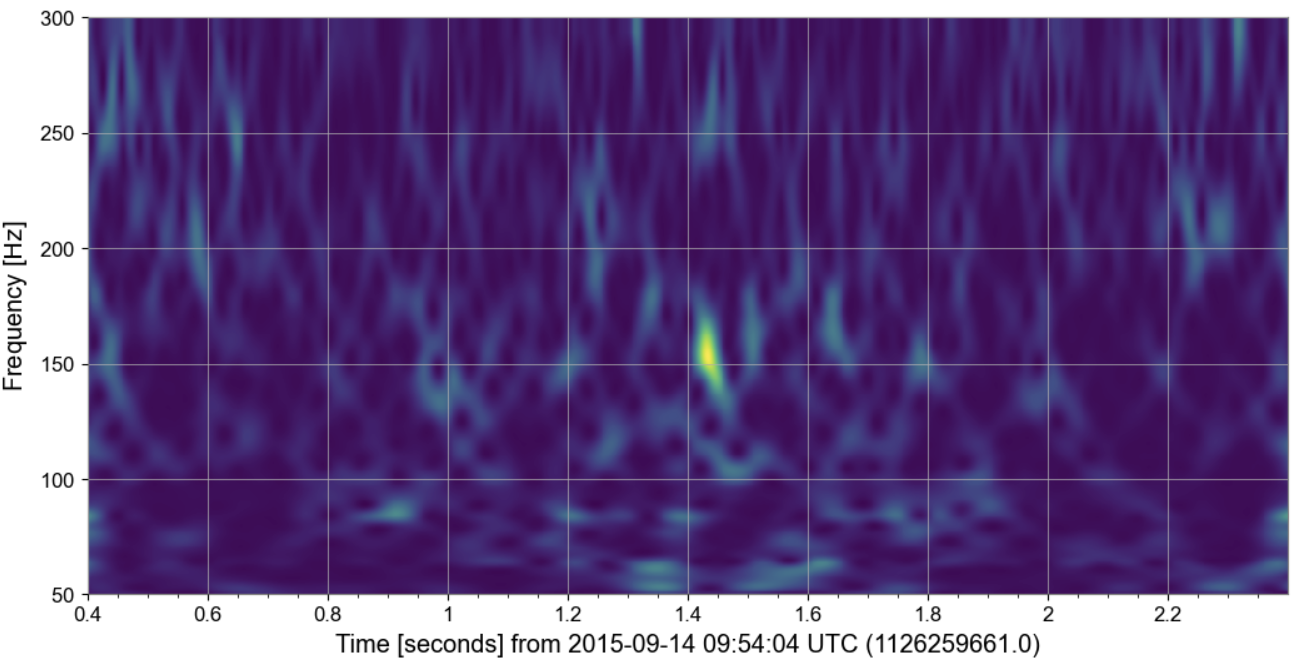
\includegraphics[width=0.9\textwidth]{figure/Qspectrogram_offsource}
	\caption{Off-source Q-transformation, showing no pattern in it.}
	\label{Qtransformation Offsource}
\end{figure}
\subsection{Key Result}

The time--frequency representation clearly demonstrates a monotonic increase in frequency and amplitude consistent with inspiral, merger, and ringdown. The morphology of the chirp provides direct evidence that the source is a compact binary system and is incompatible with stationary or broadband instrumental noise. You can see consistency between whiten data and Q-transformation from fig \ref{filtered data} and \ref{Qtransformation}.

\section{Matched Filtering, Signal-to-Noise Ratio, And $\chi$ Square} \label{sec:6}

\subsection{Matched Filtering}

We apply frequency-domain matched filtering to the H1 strain data
using waveform templates generated with the IMRPhenomD approximant.
The matched-filter SNR is defined by the noise-weighted inner product.

\begin{equation}
	(a|b) = 4 \, \Re \int_{0}^{\infty}
	\frac{\tilde{a}(f)\tilde{b}^*(f)}{S_n(f)} \, df ,
\end{equation}

where $S_n(f)$ is the one-sided power spectral density (PSD) and $\tilde{a(f)}, \tilde{b^*(f)}$ are representing detector and model data in frequency. 
The time-dependent SNR is

\begin{equation}
	\rho(t) = \frac{(s|h_t)}{\sqrt{(h|h)}} ,
\end{equation}

with $h_t$ the time-shifted template.
Inverse PSD weighting suppresses noisy frequency bands and
optimally accumulates signal power in the sensitive band
(20--300 Hz). This procedure is just like whitening data.
SNR is just: weighted dot product of signal and template.

But in discrete form the matched-filter SNR is defined:
\begin{equation}
	(a|b) = 4 \Re \sum_{k} \frac{\tilde{a}_k \tilde{b}_k^*}{S_n(f_k)} \Delta f .
\end{equation}
When we convert time-series data to frequency domain using FFT, we do not get continuous frequencies.
We get discrete frequency bins $f_k = k \Delta f$. and $\Delta f$ is resolution of our FFT and it relates to segment length. it could be calculated by dividing sample rate by length of data. 
 
\subsection{Chi-Square Signal Consistency Test}
To test waveform consistency, we compute the
power $\chi^2$ discriminator \cite{Allen2005Chisq}.
The template is divided into $p$ frequency bins,
and deviations of observed power from the expected template
distribution are measured:

\begin{equation}
	\chi^2(t) = \sum_{k=1}^{p} {\left| \rho_k(t) - \frac{\rho(t)}{p} \right|^2} ,
\end{equation}
where $\rho_k(t)$ is SNR contribution from bin k and $\rho(t)$ is total SNR. In above equation we just compare SNR of each bin with SNR that it is distributed equally between all bins. 
with degrees of freedom
\begin{equation}
	\mathrm{DOF} = 2p - 2 .
\end{equation}
we can define and use $\chi^2_{reduced}$
\begin{equation}
	\chi^2_{\mathrm{red}} = \frac{\chi^2}{\mathrm{DOF}} .
\end{equation}
In our processing if $\chi^2_{red}$ is between 1 and 2 our signal is very good.

\subsection{Reweighted SNR}

Following standard LIGO practice \cite{Allen2005Chisq, Abbott2016Discovery},
we compute the reweighted SNR:
\begin{equation}
	\hat{\rho} =
	\begin{cases}
		\rho & \text{if } \chi^2_{\mathrm{red}} \le 1, \\
		\displaystyle
		\frac{\rho}{\left[\frac{1 + (\chi^2_{\mathrm{red}})^3}{2}\right]^{1/6}}
		& \text{if } \chi^2_{\mathrm{red}} > 1.
	\end{cases}
\end{equation}

This suppresses triggers caused by noise transients that
produce large $\chi^2$ values.

\subsection{Parameter Optimization And Final Results}

We explored a small grid around the expected GW150914 masses:

\[
(m_1, m_2) \in
\{(35.5,30.5), (36,30), (36.5,30), (36,30.5), (35,30)\} M_\odot
\]

and tested $p = 16, 26, 36$ $\chi^2$ bins. The smallest reduced $\chi^2$ was obtained for:

\begin{table}[h]
	\centering
	\begin{tabular}{ll}
		$m_1 = 35.5 M_\odot$          & $\chi^2 = 147.01$ \\
		$m_2 = 30.5 M_\odot$          & Reduced $\chi^2 = 2.10$ \\
		$p = 36$ bins                 & Reweighted SNR: $\hat{\rho} = 13.31$ \\
		Peak SNR: $\rho = 17.48$      & Time offset: $29.20$ ms \\
	\end{tabular}
\end{table}
with total mass $66.0 M_\odot$ and mass ratio $q = 1.16$.

\begin{figure}[h]
	\centering
	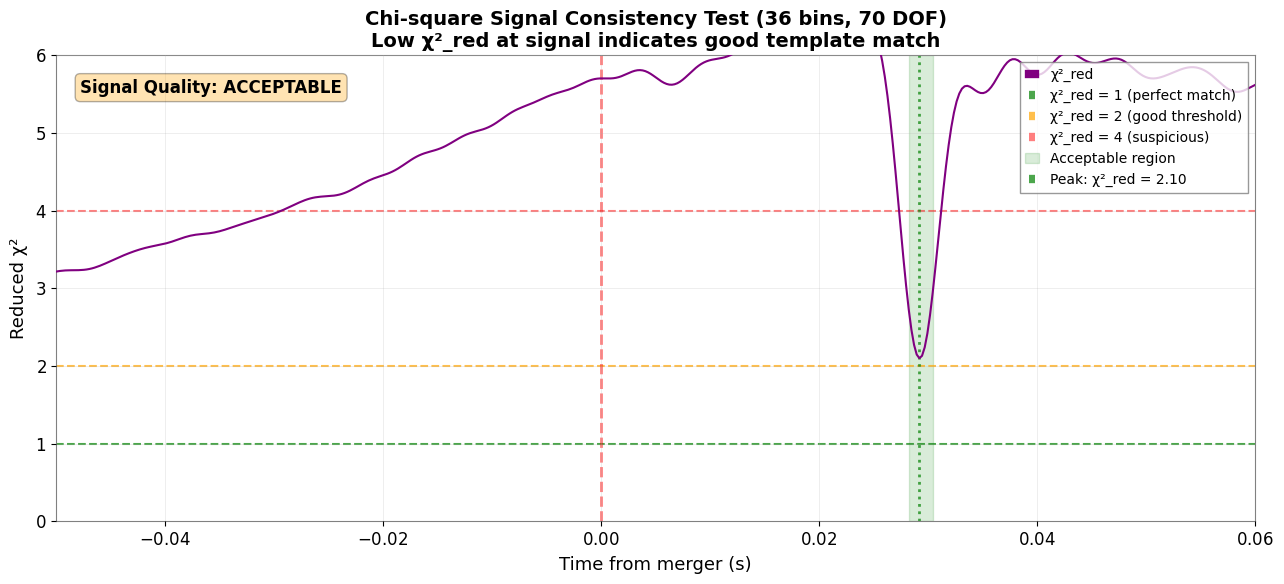
\includegraphics[width=0.9\textwidth]{figure/reduced_chi_time.png}
	\caption{$\chi^2_{red}$ over time near merger.}
	\label{chi2}
\end{figure}

The reduced $\chi^2$ indicates moderate deviation from a
perfect template match but remains within acceptable limits.
The reweighted SNR of $\hat{\rho} \approx 13.3$
corresponds to a detection significance of approximately
$13\sigma$ in Gaussian noise.
\begin{figure}[h]
	\centering
	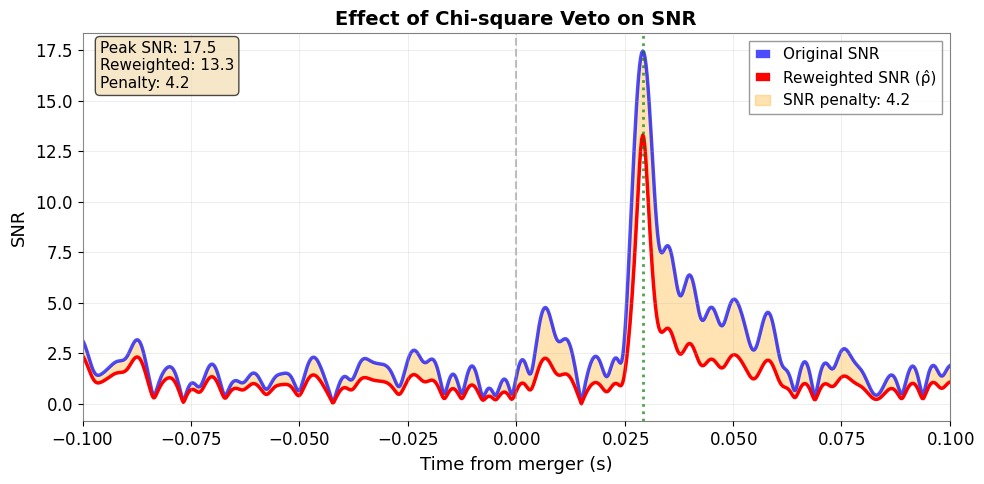
\includegraphics[width=0.9\textwidth]{figure/SNR.png}
	\caption{SNR over time near merger.}
	\label{SNR}
\end{figure}

As we see in figure \ref{chi2} and \ref{SNR}, the SNR peak completely match with best value of $\chi^2$. The "offset" refers to the time difference between where we expected the merger to occur and where we actually detected the peak signal. And For GW150914:
\begin{itemize}
	\item The entire inspiral-merger-ringdown signal lasts ~0.2 seconds
	\item A 30ms offset is only 0.15 of the total signal duration
	\item LIGO's timing accuracy is ~1-10 milliseconds, so 30ms is reasonable	
\end{itemize}
There is a offset because the merger time is not necessarily the exact moment of peak amplitude so different conventions exist for defining "merger time". Besides that IMRPhenomD is just an approximate model.

These results are consistent with the published
GW150914 analysis and confirm the astrophysical
origin of the signal.

\section{Discussion}

The analysis presented demonstrates the detection of GW150914 using open LIGO data. The measured time delay between the H1 and L1 detectors, approximately 7 ms, is consistent with the light-travel time across the Earth, confirming the coherence of the signal across detectors. Time–frequency analysis using the Q-transform reveals the characteristic chirp of a binary black hole merger, with increasing frequency and amplitude, which is consistent with theoretical predictions. 

Matched filtering with an optimized waveform template yields a peak reweighted SNR of approximately 13.3, indicating a strong detection well above noise fluctuations. The reweighted SNR incorporates the results of the $\chi^2$ signal consistency test, which measures deviations from the template and helps mitigate the influence of transient noise. The best-matching template corresponds to component masses $M_1 = 35.5 M_\odot$ and $M_2 = 30.5 M_\odot$, resulting in a total mass of $66 M_\odot$, in agreement with published results \cite{Abbott2016Discovery}. The reduced $\chi^2$ value of 2.10 indicates an acceptable agreement between the data and the template, confirming the astrophysical origin of the signal with a detection significance of roughly 13$\sigma$.

Although the $\chi^2$ test helps suppress spurious noise contributions, residual short-duration noise transients, or glitches, may still affect the data. Future analysis could focus on additional noise mitigation techniques, such as vetoing coincident triggers in auxiliary channels or applying machine learning-based classifiers to identify and remove glitches before matched filtering. Such improvements would increase the robustness of gravitational-wave detections and enhance confidence in low-SNR events.

Overall, the combination of time–frequency and matched-filter analyses provides a reliable confirmation of GW150914 and demonstrates the effectiveness of open data analysis tools for gravitational-wave astrophysics.


\bibliographystyle{unsrt}
\bibliography{references} % see references.bib for bibliography management

\end{document}
